% Chapter 15 -- Claim: Black--Scholes Delta Hedging Removes Option Risk
% Requires: amsmath, amssymb, booktabs, array, tabularx, graphicx, tcolorbox (breakable, skins), hyperref or url.
% Defines the callout box only if the preamble has not.
\providecolor{fenavy}{HTML}{1B2A6B}
\providecolor{feshade}{HTML}{F3F5FA}
\makeatletter
\@ifundefined{callout}{%
  \newtcolorbox{callout}{breakable, enhanced,
    colback=white, colframe=gray!70, boxrule=0.5pt, arc=1mm,
    borderline west={2.5pt}{0pt}{gray!70},
    left=8pt, right=8pt, top=4pt, bottom=4pt}%
}{}
\makeatother

\chapter{Claim: Black--Scholes Delta Hedging Removes Option Risk}
\label{ch:15}

The Black--Scholes--Merton model rests on a striking claim: an option can be manufactured. By holding the right number of shares and adjusting that number continuously, a trader can reproduce the option's payoff exactly, whatever the market does. If that is true, the option's price is not a matter of opinion about where the market is going. It is the cost of the recipe. A dealer who sells an option at that price and follows the recipe is left with no risk.

The argument transformed finance. It created the options industry, it underpins the pricing of almost every derivative, and it is why banks can sell structured products and hedge them rather than bet on them. Chapter 14 asked whether option sellers earn a premium. This chapter asks something more basic: does the recipe work? When a seller hedges as the model prescribes, on real market paths, how much risk is actually left?

By the end of the chapter you will be able to:

\begin{itemize}
  \item explain the replication argument behind Black--Scholes and the assumptions it needs;
  \item decompose a delta-hedged option's daily P\&L into gamma and theta, and compute the break-even daily move;
  \item estimate the error from hedging at discrete intervals, and explain why it shrinks with the square root of the hedging frequency;
  \item explain the volatility smile and why it is evidence against the model's assumptions;
  \item state the claim that delta hedging removes option risk, and test it by hedging along real and simulated market paths;
  \item judge what risks a ``fully hedged'' option seller or structured-product issuer still carries.
\end{itemize}

\section{Foundations: replication and the Greeks}
\label{sec:15-foundations}

\textbf{Replication.} Black and Scholes (1973) and Merton (1973) assumed that the stock price follows a geometric Brownian motion with constant volatility $\sigma$, that trading is continuous and costless, and that the risk-free rate is constant. Under those assumptions, a portfolio of $\Delta = \partial V/\partial S$ shares and a bond, rebalanced continuously, has exactly the same value as the option at every moment. Because the option can be replicated, its price must equal the cost of the replicating portfolio. Otherwise there would be an \textbf{arbitrage}, a riskless profit. The resulting price depends on $\sigma$ but not on the stock's expected return.

\textbf{Delta hedging} is the same recipe run in reverse. A dealer who sells an option holds $\Delta$ shares to offset it. Over a short interval, the option's value changes by roughly
\begin{equation}
  dV \approx \Delta\,dS + \tfrac{1}{2}\Gamma\,dS^2 + \Theta\,dt
  \label{eq:15-taylor}
\end{equation}
where:

\begin{itemize}
  \item $\Delta$ (\textbf{delta}) is the first-order sensitivity to the stock price, which the shares offset;
  \item $\Gamma$ (\textbf{gamma}) is the curvature, $\partial^2 V/\partial S^2$, which the shares cannot offset;
  \item $\Theta$ (\textbf{theta}) is the time decay, which the option seller earns.
\end{itemize}

\textbf{The hedging P\&L.} For a seller who hedges at the implied volatility $\sigma$, the profit over one day is approximately
\begin{equation}
  \text{P\&L} \approx \tfrac{1}{2}\,\Gamma S^2 \left(\sigma^2 \Delta t - r^2\right)
  \label{eq:15-pnl}
\end{equation}
where $r$ is that day's return and $\Delta t$ is one day as a fraction of a year. The seller earns theta on quiet days and loses on days when the stock moves more than the implied volatility predicts. Summed over the option's life, the hedged P\&L is a gamma-weighted bet that realized variance will be below implied variance. In the Black--Scholes world, realized variance equals $\sigma^2$ on average, so the bet is fair and, with continuous hedging, riskless.

\textbf{Discrete hedging.} Real hedgers rebalance at intervals. Even in the Black--Scholes world this leaves an error whose standard deviation falls with the square root of the number of rebalances. Kamal and Derman (1999) showed that for an at-the-money option hedged $N$ times it is about
\begin{equation}
  \mathrm{sd}(\text{hedging error}) \approx \sqrt{\frac{\pi}{4}}\;\frac{\sigma \times \text{vega}}{\sqrt{N}}
  \label{eq:15-kd}
\end{equation}
where vega is measured per unit of $\sigma$. That is about a fifth of the premium for a one-month option hedged daily. Quadrupling the hedging frequency halves the error (Figure~\ref{fig:15-freq}).

\begin{figure}[htbp]
\centering
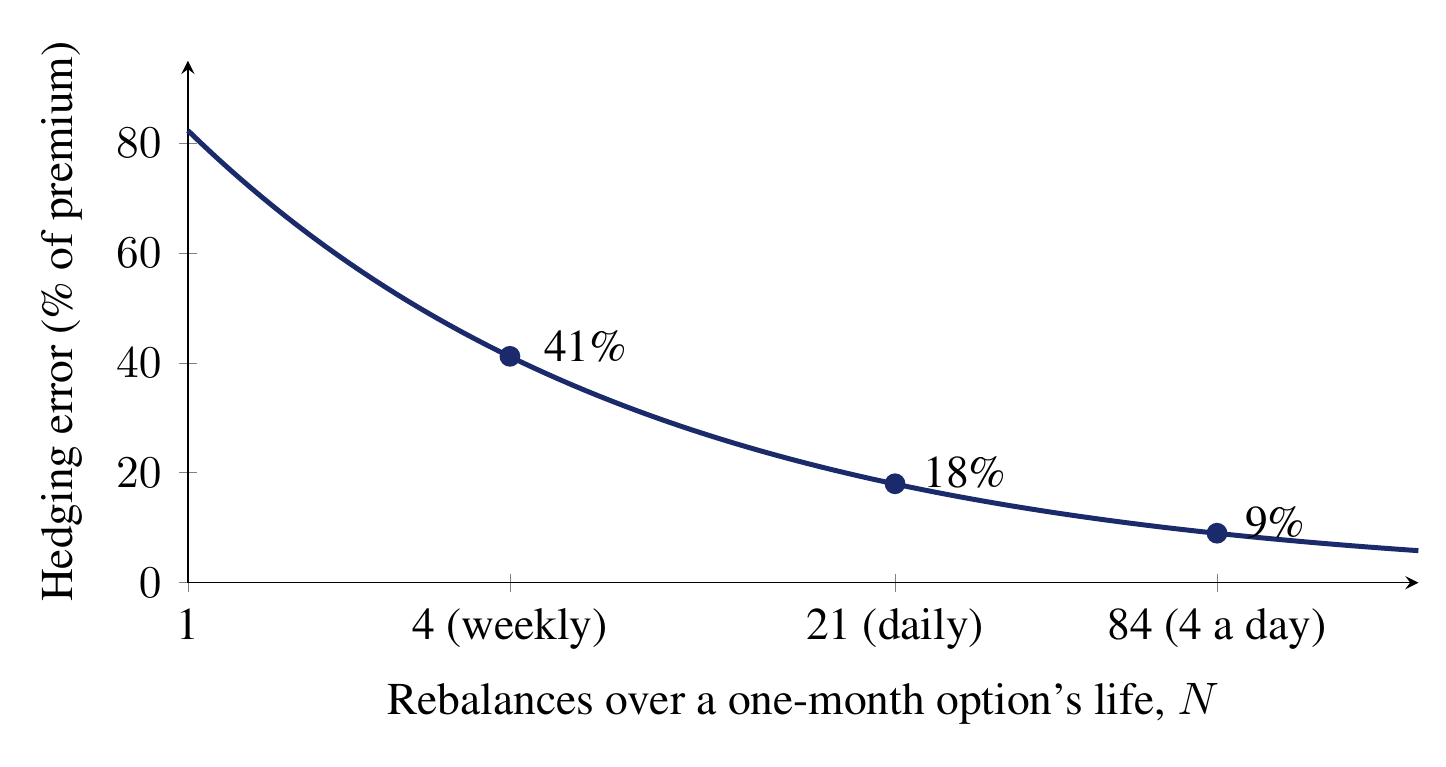
\includegraphics[width=0.85\linewidth]{images/fig15-1-hedge-frequency.png}
\caption{Hedging error in the Black--Scholes world, by the Kamal--Derman approximation, for a one-month at-the-money option at 20\% volatility. Hedging weekly leaves an error of about 41\% of the premium, daily about 18\%, and four times a day about 9\%. Each quadrupling of the frequency halves the error.}
\label{fig:15-freq}
\end{figure}

\textbf{The volatility smile.} If Black--Scholes were right, every option on the same asset would have the same implied volatility. In practice, implied volatility varies with the strike: for stock indexes, low-strike puts trade at much higher implied volatilities than at-the-money options. This \textbf{skew} or \textbf{smile} is the market's admission that returns are not lognormal with constant volatility.

\textbf{Worked example.} The index is at 100, the risk-free rate is 4\%, and a one-month at-the-money call is sold at 20\% implied volatility (Figure~\ref{fig:15-pnl}).

\begin{itemize}
  \item Price \$2.47, delta 0.53, gamma 0.069, theta $-\$0.063$ a day. The dealer sells the call and buys 0.53 units of the index.
  \item If the index is unchanged the next day, the dealer earns the theta: about \$0.063.
  \item If the index moves 3 points either way, the gamma loss is $\tfrac{1}{2} \times 0.069 \times 3^2 = \$0.31$, and the dealer loses about $\$0.31 - \$0.063 = \$0.25$ before rebalancing.
  \item The break-even daily move is $\sqrt{2 \times 0.063/0.069} \approx 1.35$ points, close to the 1.26-point daily standard deviation that 20\% annual volatility implies. Hedging is a wager that daily moves will average less than that.
\end{itemize}

\begin{figure}[htbp]
\centering
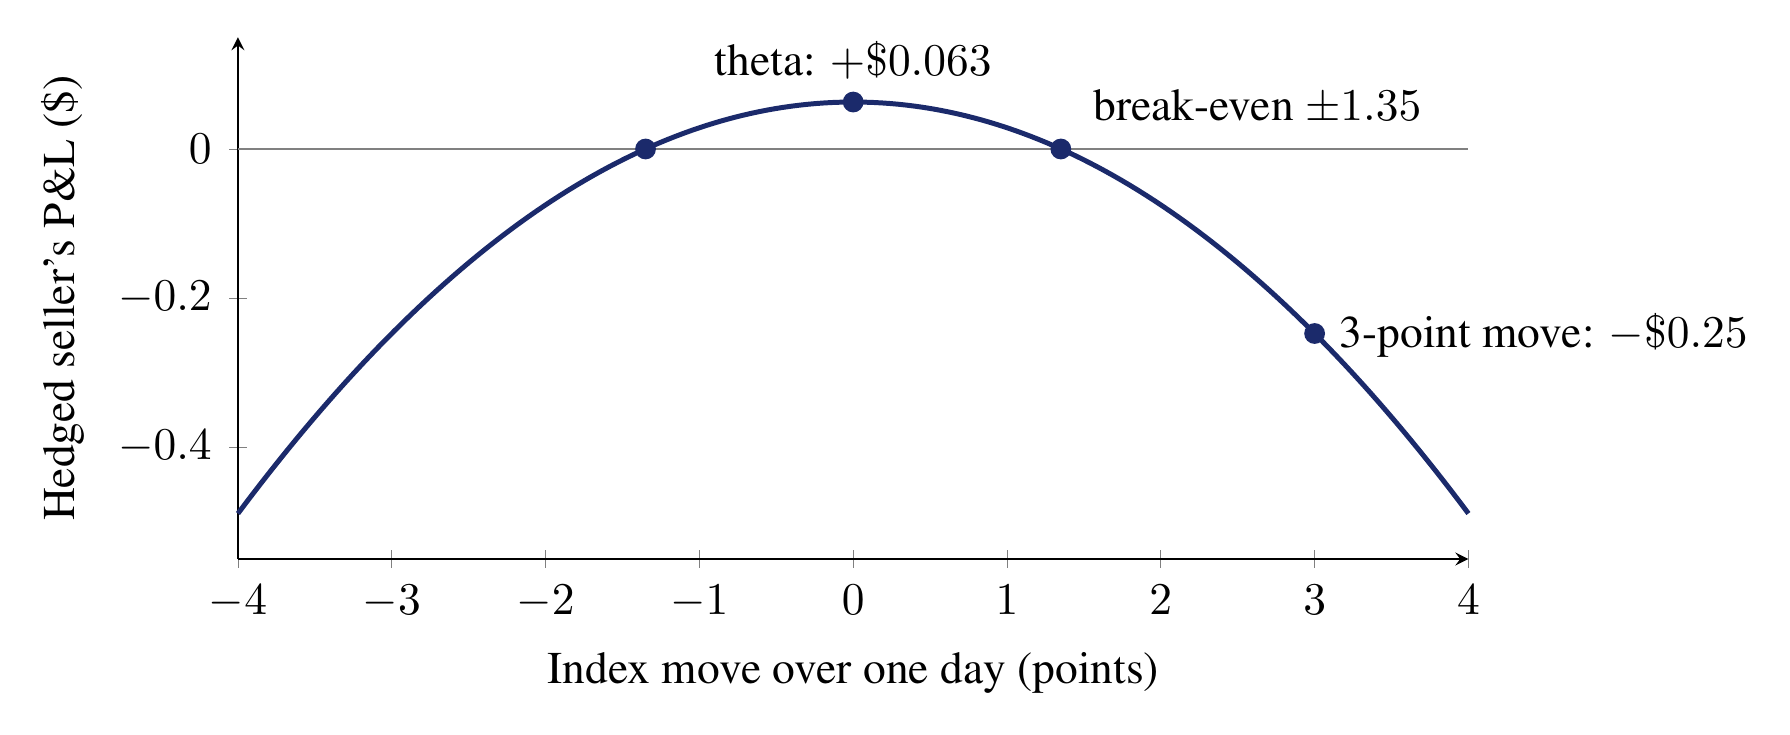
\includegraphics[width=0.85\linewidth]{images/fig15-2-hedge-pnl.png}
\caption{The delta-hedged call seller's P\&L over one day in the worked example. The seller earns \$0.063 of theta if the index is unchanged, breaks even on a move of about 1.35 points either way, and loses \$0.25 on a 3-point move. The loss grows with the square of the move.}
\label{fig:15-pnl}
\end{figure}

\textbf{Further reading.} Hull, \emph{Options, Futures, and Other Derivatives} (the Black--Scholes--Merton model, the Greeks, delta hedging, volatility smiles); Wilmott, \emph{Paul Wilmott Introduces Quantitative Finance} (hedging and the hedging P\&L); Shreve, \emph{Stochastic Calculus for Finance II} (replication); Gatheral, \emph{The Volatility Surface}.

\section{How it works}
\label{sec:15-how}

The replication argument can fail in four ways, and each leaves a different fingerprint on the hedging P\&L.

\begin{center}
\small
\begin{tabularx}{0.9\linewidth}{@{}>{\raggedright\arraybackslash}p{0.2\linewidth}>{\raggedright\arraybackslash}X>{\raggedright\arraybackslash}X@{}}
\toprule
Assumption & What happens in practice & Effect on a hedged option seller \\
\midrule
Continuous trading & Hedgers rebalance daily or less often & Random errors that shrink with hedging frequency; present even when the model is right \\
Constant, known volatility & Volatility changes and clusters (Chapter 11) & P\&L tracks realized minus implied variance; losses when volatility rises \\
Continuous price paths & Prices jump, as in October 1987 or March 2020 & Large losses on jump days that no rebalancing frequency can prevent \\
No trading costs & Every rebalance pays a spread & A steady drag that grows with hedging frequency \\
\bottomrule
\end{tabularx}
\end{center}

The first is a property of the model itself: it would occur even if Black--Scholes were exactly right. The others are failures of its assumptions. A test of the claim must separate them, and the cleanest way is to run the same hedging strategy twice, once on real market paths and once on simulated paths that obey the model exactly. The difference between the two is the cost of the model's being wrong.

\textbf{Jumps are the hardest problem.} Over a day in which the market falls 20\%, the change in the option's value is far from the delta-hedge's change. The gamma term $\tfrac{1}{2}\Gamma\,dS^2$ is enormous, and rebalancing more often does not help, because the jump happens between rebalances. A seller of options is short gamma, so a jump in either direction is a loss.

\textbf{Volatility changes} are a second-order version of the same problem. If realized volatility over the month is twice the implied volatility used to price and hedge the option, the seller loses roughly vega times the gap, regardless of how often the hedge is adjusted.

\textbf{The smile is the market's response.} After October 1987, dealers began to charge more for the risks that delta hedging cannot remove: crashes and volatility spikes. They did so by raising the implied volatility of out-of-the-money puts, the options that pay off in crashes. The smile is thus both evidence against the Black--Scholes assumptions and the price of the residual risk that delta hedging leaves.

\section{The claim}
\label{sec:15-claim}

\begin{callout}
\textbf{Claim.} An option seller who delta-hedges as Black--Scholes prescribes is left with little risk. Hedging removes most of the variance of the unhedged position, and what remains is small, symmetric and shrinks as hedging becomes more frequent.
\end{callout}

This is the claim that justifies treating an option's Black--Scholes price as its cost of production. To test it we need to be precise on four points.

\begin{itemize}
  \item \textbf{Little risk relative to what.} The benchmark is the unhedged short option. A hedge that removes 90\% of its variance and leaves errors of a fifth of the premium, as in the Black--Scholes world with daily hedging, meets the claim. A hedge that leaves occasional losses of several times the premium does not.
  \item \textbf{Which volatility.} The seller must price and hedge at some volatility. We use the VIX, the market's implied volatility, so the test is whether hedging at the market's price leaves little risk.
  \item \textbf{Which statistic.} The standard deviation of the hedging error captures day-to-day risk. The 1\% quantile and the worst month capture tail risk. The claim requires both to be small.
  \item \textbf{What would count against it.} The claim fails if hedging on real paths leaves much more risk than on Black--Scholes paths, if the remaining errors are fat-tailed, or if more frequent hedging fails to reduce them.
\end{itemize}

\section{The original evidence}
\label{sec:15-evidence}

\textbf{The model.} Black and Scholes (1973) derived the option price from a hedging argument, and Merton (1973) generalized it and set out the conditions under which it holds. Early empirical tests, including their own (Black and Scholes 1972), found the model a useful approximation with systematic deviations from market prices. Within a few years Black--Scholes prices and deltas were standard on trading floors.

\textbf{Transaction costs.} Leland (1985) showed that with proportional trading costs, perfect replication is impossible: hedging continuously would cost an infinite amount. He proposed hedging at discrete intervals with an adjusted volatility, raised for an option seller to cover the expected costs, and showed that the adjustment grows as the hedging interval shrinks. Even in principle, the seller faces a trade-off between hedging error and trading costs.

\textbf{The smile after 1987.} Rubinstein (1994) documented that before October 1987, implied volatilities of S\&P 500 index options were roughly the same across strikes, as Black--Scholes requires. After the crash, a pronounced skew appeared, with low-strike puts priced at much higher implied volatilities, and it has persisted ever since. He developed implied binomial trees to fit it. The smile is direct evidence that the market does not price options as if Black--Scholes held.

\textbf{Better models.} Bakshi, Cao and Chen (1997) tested models with stochastic volatility, jumps and stochastic interest rates on S\&P 500 options. Adding stochastic volatility and jumps improved pricing. For hedging, modelling stochastic volatility alone gave the best performance; jumps helped pricing but not hedging, because a jump cannot be hedged with the underlying asset at all.

\textbf{Portfolio insurance.} The most consequential test of dynamic replication was not an academic study. In the 1980s, portfolio insurance programmes used dynamic trading in index futures to replicate a protective put on large equity portfolios. The Brady Commission (Presidential Task Force on Market Mechanisms 1988) estimated that \$60 to \$90 billion of equity assets were under portfolio insurance when the market crashed in October 1987. The What Failed box in Section~\ref{sec:15-investors} tells what happened.

\section{Replication lab: hedging options along real paths}
\label{sec:15-lab}

\begin{callout}
\textbf{Lab 15 at a glance.} \emph{Claim on trial:} delta hedging removes option risk. \emph{Data:} daily market returns from the Kenneth French library and the VIX from FRED, from 1990; both are free. \emph{Code:} runs as a script (\texttt{python lab15.py}) or as a notebook with a prediction prompt before each step.
\end{callout}

At each month end the lab sells a one-month at-the-money call on the market at its Black--Scholes price, using the VIX as the implied volatility. It buys $\Delta$ units of the index, finances them at the risk-free rate, rebalances on a schedule, and pays the option's payoff at expiry. The final value is the \textbf{hedging P\&L}, expressed as a share of the premium. The same strategy is then run on 20 simulated geometric Brownian motion paths per month, using that month's implied volatility, where the Black--Scholes assumptions hold exactly.

\textbf{Part A, residual risk.} Mean, standard deviation, skewness, 1\% quantile and worst month of the hedged P\&L for daily, two-day, weekly, two-weekly and no hedging, on real and simulated paths, and the share of the unhedged risk removed (Figure 15.3).

\textbf{Part B, source.} A regression of the actual P\&L on the gamma--theta approximation of Equation~\eqref{eq:15-pnl} summed over the month (Figure 15.5), and on the gap between implied and realized variance.

\textbf{Part C, frictions.} Hedging frequency (Figure 15.6) and transaction costs of 0 to 10 basis points per unit of index traded (Figure 15.7).

\textbf{Part D, tail.} The worst months, with the market move, implied and realized volatility and the largest daily move, and the share of all losses that came from the worst 5\% of months (Figure 15.4).

Two design choices matter for interpretation. First, pricing at the VIX overstates at-the-money implied volatility, as Chapter 14 explained, so the \emph{mean} hedged P\&L includes the variance risk premium plus some overstatement. The \emph{spread} of the P\&L, which is what the claim is about, is little affected. Second, a delta-hedged call and a delta-hedged put with the same strike are the same position, so the lab uses calls only.

\textbf{What the simulated run shows.} On the simulated Black--Scholes paths, daily hedging leaves a mean P\&L near zero and a standard deviation of about 17\% of the premium, in line with the Kamal--Derman formula, and the error falls steadily as hedging becomes more frequent. On the simulated GARCH paths with fat tails, which play the role of real paths in the test run, daily hedging still removes most of the unhedged risk. But the residual is larger, negatively skewed and concentrated: the worst 5\% of months produced most of the losses. The gamma--theta approximation explains most of the P\&L, and the largest deviations from it come in months with big daily moves. These results confirm that the code works. They say nothing about real markets. Run the lab on the real data to reach your own verdict.

\section{Stress tests}
\label{sec:15-stress}

\textbf{Hedging frequency.} In the Black--Scholes world, hedging four times as often halves the error (Figure~\ref{fig:15-freq}). On real paths, the part of the error that comes from discrete rebalancing falls in the same way, but the parts that come from jumps and volatility changes do not. If the lab finds that moving from weekly to daily hedging reduces risk much less on real paths than on simulated ones, the residual is dominated by risks that rebalancing cannot remove.

\textbf{Transaction costs.} Every rebalance pays a spread. With costs of a few basis points per unit of index traded, daily hedging can consume a large share of the seller's margin, which is why dealers hedge less often than the model prescribes and why Leland's adjusted volatility exists. The lab's cost experiment shows how quickly the trade-off bites.

\textbf{Crash months.} The months that matter are those with jumps: October 1987 (before the lab's sample), August 1998, October 2008, August 2011, August 2015, February 2018 and March 2020. In each, a one-month option sold at the start of the month at the prevailing implied volatility faced daily moves far larger than that volatility implied. Expect the hedged seller's worst months to be these, with losses of a multiple of the premium even with daily hedging.

\textbf{Realized versus implied volatility.} The gamma--theta approximation says the hedged P\&L is a bet that realized variance will be below implied. When implied volatility is above realized, as it is in most months (Chapter 14), the hedged seller earns a profit. That profit is not evidence that hedging removed risk. It is the variance risk premium, earned by bearing the risk that remains. A hedge that leaves a positive mean and a fat left tail has turned an option position into a short-volatility position, not into a riskless one.

\textbf{Model risk in the hedge ratio.} Black--Scholes deltas assume volatility does not change when the price moves. For stock indexes, volatility tends to rise when prices fall (Chapter 11). Hull and White (2017) showed that adjusting the delta for this relation, a \textbf{minimum-variance delta}, reduces hedging errors for index options. The size of the improvement is itself a measure of how wrong the Black--Scholes hedge ratio is.

\section{Verdict}
\label{sec:15-verdict}

\begin{callout}
\textbf{Verdict: fails as a description of practice} (as of October 2026). Black--Scholes delta hedging removes most of the day-to-day risk of an option position, but what it leaves is not little and not symmetric. The residual is a bet on realized versus implied volatility, with fat-tailed losses in months with jumps and volatility spikes, and those losses cannot be eliminated by hedging more often.
\end{callout}

What survives:

\begin{itemize}
  \item \textbf{Delta hedging works as a first approximation.} It removes most of the variance of an unhedged option position. It is the reason dealers can sell options without betting on market direction, and the reason Black--Scholes remains the industry's common language, even as a quoting convention.
  \item \textbf{The hedging P\&L is understood.} The gamma--theta approximation explains most of it. A trader knows what bet the hedged book contains: short realized volatility, long implied.
\end{itemize}

What fails:

\begin{itemize}
  \item \textbf{The residual is large and fat-tailed.} On real paths, hedging leaves more risk than on Black--Scholes paths, and the worst months bring losses of a multiple of the premium.
  \item \textbf{More frequent hedging cannot fix it.} Jumps happen between rebalances. Volatility changes are not hedged by the underlying at all. Hedging more often raises costs without removing these risks.
  \item \textbf{The market knows.} The volatility smile that has existed since 1987 is the market's price for the risks delta hedging leaves. If the claim were true, the smile would not exist.
\end{itemize}

The verdict would move to \emph{weakens} if a simple extension, such as hedging with a minimum-variance delta or adding a small position in other options to hedge vega and gamma, removed most of the tail. That is how dealers actually hedge, and it is why they never rely on delta alone.

\section{What investors can use}
\label{sec:15-investors}

\textbf{The residual risks inside structured products.} A bank that sells a structured note with a capped equity return or a principal guarantee is short options, and it hedges them dynamically. The hedge removes most of the market risk, but the bank keeps the risks this chapter identifies: jumps, volatility changes and the cost of rebalancing. It charges for them, which is part of why such products are expensive. When an investor buys one, the fee includes the price of risks the bank cannot hedge away.

\textbf{Option-based funds.} A fund that sells options and delta-hedges them is not market-neutral in the sense that matters. It is short volatility: it earns steady returns in calm markets and loses heavily in jumps. Its track record will look smooth until a crash.

\textbf{Why the smile exists.} The higher implied volatility of out-of-the-money index puts is not a quirk. It is the price of crash risk, which delta hedging cannot remove. An investor buying downside protection pays it; an investor selling protection is paid it for bearing the jumps.

\textbf{Questions to ask a manager or a structured-product issuer:}

\begin{itemize}
  \item How are the option positions hedged: delta only, or also vega and gamma with other options?
  \item What happens to the hedge in a one-day move of 10\% or 20\%?
  \item How often is the hedge rebalanced, and what does rebalancing cost?
  \item What was the strategy's worst month, and was it in a crash?
\end{itemize}

\begin{callout}
\textbf{What Failed: portfolio insurance, October 1987.} Portfolio insurance, developed by Hayne Leland and Mark Rubinstein, replicated a protective put on an equity portfolio by dynamic trading: selling stock-index futures as the market fell and buying them back as it rose, exactly as delta hedging prescribes. By October 1987, according to the Brady Commission, \$60 to \$90 billion of equity assets were under portfolio insurance.

On October 19, 1987, the market fell more than 20\% in a day. The strategy required insurers to sell at every step down. According to the Brady Commission, portfolio insurers sold the equivalent of about \$4 billion of stock in index futures, more than 40\% of futures volume excluding locals' trades, and just under \$2 billion of stock directly on the New York Stock Exchange. Prices moved faster than the trades could be executed, so the hedge was always behind. Insurers could not trade at the prices their models assumed, so the protection they delivered fell short of the puts they were replicating, and the Brady Commission concluded that their mechanical selling added to the pressure on prices.

The failure was the replication assumption itself: continuous trading at continuous prices. A real put would have paid off regardless of how the market got there. A replicated put depended on trading through the fall, and the market did not allow it. The volatility skew that appeared after the crash has been the market's price for that lesson ever since.
\end{callout}

\section{Open questions}
\label{sec:15-open}

\begin{itemize}
  \item \textbf{How much of the hedging error is compensation for bearing jump risk?} If the mean hedged P\&L of option sellers is positive, is it just enough to pay for the jumps, or more?
  \item \textbf{How much better do practical hedges do?} Minimum-variance deltas, vega hedges with other options and stochastic-volatility models all reduce hedging error. How much of the tail do they remove on real paths?
  \item \textbf{Do short-dated options change the picture?} Options expiring within a day have enormous gamma near expiry. Does dealers' hedging of them amplify intraday moves?
  \item \textbf{Can machine-learning hedges beat Black--Scholes?} ``Deep hedging'' learns hedging rules directly from data with costs and constraints. Do its gains survive out of sample and in crashes?
\end{itemize}

\section*{Exercises}
\addcontentsline{toc}{section}{Exercises}

\subsection*{Conceptual (all readers)}

\begin{enumerate}
  \item For the worked example in Section~\ref{sec:15-foundations}, compute the hedged seller's P\&L over one day if the index moves 1, 2 and 4 points. At what daily move does the seller break even?
  \item Using the Kamal--Derman approximation, Equation~\eqref{eq:15-kd}, compute the standard deviation of the hedging error, as a share of the premium, for a one-month at-the-money option hedged daily, weekly and four times a day.
  \item Show that a delta-hedged call and a delta-hedged put with the same strike and expiry have the same hedged P\&L.
\end{enumerate}

\subsection*{Lab extensions (technical readers)}

\begin{enumerate}
  \setcounter{enumi}{3}
  \item Part A: compare the share of unhedged risk removed by daily hedging on real and Black--Scholes paths. Compare the 1\% quantiles. Which comparison is more informative about the claim?
  \item Part B: what share of the variance of the hedged P\&L does the gamma--theta approximation explain? Find the months with the largest residuals. What happened in them?
  \item Part C: at what transaction cost does weekly hedging give a higher mean P\&L than daily hedging? What is the effect on the 1\% quantile?
  \item Part D: compute the share of all hedging losses that came from the worst 5\% of months. Compare it with the Black--Scholes paths.
  \item Price the option at the VIX but hedge using trailing 21-day realized volatility. How does the P\&L distribution change?
  \item A structured-product salesperson says the bank's position is ``fully hedged.'' Using this chapter's evidence, explain what risks the bank still carries and how it charges for them.
\end{enumerate}

\section*{References}
\addcontentsline{toc}{section}{References}

\begin{itemize}
  \item Bakshi, G., Cao, C. and Chen, Z. (1997). Empirical Performance of Alternative Option Pricing Models. \emph{Journal of Finance} 52(5): 2003--2049.
  \item Black, F. and Scholes, M. (1972). The Valuation of Option Contracts and a Test of Market Efficiency. \emph{Journal of Finance} 27(2): 399--417.
  \item Black, F. and Scholes, M. (1973). The Pricing of Options and Corporate Liabilities. \emph{Journal of Political Economy} 81(3): 637--654.
  \item Hull, J. and White, A. (2017). Optimal Delta Hedging for Options. \emph{Journal of Banking \& Finance} 82: 180--190.
  \item Kamal, M. and Derman, E. (1999). When You Cannot Hedge Continuously: The Corrections to Black--Scholes. \emph{Risk} 12(1).
  \item Leland, H. E. (1985). Option Pricing and Replication with Transactions Costs. \emph{Journal of Finance} 40(5): 1283--1301.
  \item Merton, R. C. (1973). Theory of Rational Option Pricing. \emph{Bell Journal of Economics and Management Science} 4(1): 141--183.
  \item Presidential Task Force on Market Mechanisms (1988). \emph{Report of the Presidential Task Force on Market Mechanisms} (the Brady Report). Washington, DC: U.S. Government Printing Office.
  \item Rubinstein, M. (1994). Implied Binomial Trees. \emph{Journal of Finance} 49(3): 771--818.
\end{itemize}

\textbf{Data:} Kenneth R. French Data Library, Fama/French 3 Factors [Daily]. Chicago Board Options Exchange, CBOE Volatility Index: VIX [VIXCLS], retrieved from FRED, Federal Reserve Bank of St.\ Louis.
